%\documentclass[handout]{beamer}
\documentclass{beamer}
 
\usetheme[numbering = fraction, progressbar = none, background = light, sectionpage = progressbar]{metropolis}
\usepackage{amsmath}
\usepackage{synttree}
\usepackage{tabu}
\usepackage{graphicx}
\usepackage{setspace}

\title{Econ 103 -- Statistics for Economists}
\subtitle{Chapter 3: Probability}
\author{Mallick Hossain}
\date{}
\institute{University of Pennsylvania}
\begin{document} 

%%%%%%%%%%%%%%%%%%%%%%%%%%%%%%%%%%%%%%%%
\begin{frame}
	\titlepage 
\end{frame} 

\section{R Project}
%%%%%%%%%%%%%%%%%%%%%%%%%%%%%%%%%%%%%%%%
\begin{frame}
\frametitle{Motivation}
    \begin{itemize}[<+- | alert@+>]
        \item Apply the skills and tools you have learned
        \begin{itemize}
        		\item Sidebar on me and metrics
        \end{itemize}
        \item Answer questions you are interested in
        \item Head-start on honors thesis?
    \end{itemize}
\end{frame}

%%%%%%%%%%%%%%%%%%%%%%%%%%%%%%%%%%%%%%%%
\begin{frame}
\frametitle{What Subjects Can I Explore?}
    \begin{itemize}[<+- | alert@+>]
        \item ANYTHING\only<2->{, \alert<2>{seriously.}}
        \begin{itemize}
        		\item Political or ideological agendas are welcome
        		\item Guns, gender, inequality, race, climate change, \ldots
        		\item Google trends, Twitter, financial data, macro data, \ldots
        \end{itemize}
    \end{itemize}
\end{frame}

%%%%%%%%%%%%%%%%%%%%%%%%%%%%%%%%%%%%%%%%
\begin{frame}
\frametitle{What Do I Turn In?}
    \begin{itemize}[<+- | alert@+>]
        	\item Summary of question
		\item Summary of data and why it is relevant for the question			
		\item Tables and charts of summary stats of the data
		\item Data visualization/hypothesis testing
		\item Discussion of results
		\item Criticism of your findings. What are the biggest flaws in your analysis or in the underlying data?
		\item Suggestions for further analysis or extension to the project
    \end{itemize}
\end{frame}

%%%%%%%%%%%%%%%%%%%%%%%%%%%%%%%%%%%%%%%%
\begin{frame}
\frametitle{Examples}
    \begin{itemize}[<+- | alert@+>]
        	\item R Tutorials provide some examples of the kinds of exploration I am looking for
        	\item CEA blog posts on \href{https://www.whitehouse.gov/blog/2016/09/02/employment-situation-august}{jobs} and \href{https://www.whitehouse.gov/blog/2016/08/26/second-estimate-gross-domestic-product-second-quarter-2016}{GDP}
        	\item FiveThirtyEight's report on \href{http://fivethirtyeight.com/features/gun-deaths/}{gun deaths}
    \end{itemize}
\end{frame}

%%%%%%%%%%%%%%%%%%%%%%%%%%%%%%%%%%%%%%%%
\begin{frame}
\frametitle{Do I Need to Discover Something New?}
    \begin{itemize}[<+- | alert@+>]
        	\item Not looking for a Nobel-prize-winning discovery
        	\item You should learn something new
        	\item Hopefully I'll learn something new as well
        	\item Be honest
    \end{itemize}
\end{frame}

\section{Odd Questions}

\begin{singlespace}
%%%%%%%%%%%%%%%%%%%%%%%%%%%%%%%%%%%%%%%%
\begin{frame}
\frametitle{``Odd Question'' \# 1}
	Is the following likely true or false and why? 
	\begin{quote}
	    The counties with the \textbf{lowest} incidence of kidney cancer are mostly rural, sparsely 
	    populated, and located in traditionally Republican states in the Midwest, the South, and the 
	    East. 
	\end{quote}
    \only<2->{
    \begin{itemize}
        \item Less water or air pollution
        \item Lower stress
        \item Healthier food
    \end{itemize}}    	
\end{frame}

%%%%%%%%%%%%%%%%%%%%%%%%%%%%%%%%%%%%%%%%
\begin{frame}
\frametitle{``Odd Question'' \# 1}
	Is the following likely true or false and why? 
	\begin{quote}
	    The counties with the \textbf{highest} incidence of kidney cancer are mostly rural, sparsely 
	    populated, and located in traditionally Republican states in the Midwest, the South, and the 
	    East. 
	\end{quote}
    \only<2->{
    \begin{itemize}
        \item Higher stress because of poverty
        \item Drink alcohol
        \item Higher tobacco use
    \end{itemize}}    	
\end{frame}

%%%%%%%%%%%%%%%%%%%%%%%%%%%%%%%%%%%%%%%%
\begin{frame}
\frametitle{``Odd Question'' \# 1}
    Which statement is right?    
    \begin{enumerate}[<+->]
        \item Lower rate in rural counties
        \item Higher rate in rural counties
        \item \alert<5>{Both}
        \item Neither
    \end{enumerate}
\end{frame}

%%%%%%%%%%%%%%%%%%%%%%%%%%%%%%%%%%%%%%%%
\begin{frame}
\frametitle{How?}
From \textit{Thinking Fast and Slow} by Daniel Kahneman
    \begin{quote}
        Something is wrong, of course. The rural lifestyle cannot explain both very high and very low 
        incidence of kidney cancer. The key factor is not that the counties were rural or predominately 
        Republican. \alert{It is that rural counties have small populations.}
    \end{quote}
\end{frame}

%%%%%%%%%%%%%%%%%%%%%%%%%%%%%%%%%%%%%%%%
\begin{frame}
\frametitle{``Odd Question'' \# 2}
	Pia is thirty-one years old, single, outspoken, and smart. She was a philosophy major. When a 
	student, she was an ardent supporter of Native American rights, and she picketed a department 
	store that had no facilities for nursing mothers. 

    \vspace{1em}
    Rank the following statements in order from most probable to least probable.
	\begin{enumerate}[(a)]
		\item Pia is a bank teller.
		\item Pia is a bank teller and an active feminist.
	\end{enumerate}
\end{frame}

%%%%%%%%%%%%%%%%%%%%%%%%%%%%%%%%%%%%%%%%
\begin{frame}
\frametitle{The Conjunction Fallacy}
    \textbf{When it is assumed that specific conditions are more probable than a single general one.}

    Think Venn diagrams (we'll see this formally later in the lecture)
\end{frame}

%%%%%%%%%%%%%%%%%%%%%%%%%%%%%%%%%%%%%%%%
\begin{frame}
\frametitle{``Odd Question'' \# 3}
	In Lotto 6/49, a standard government-run lottery, you choose 6 out of 49 numbers (1 through 49). 
	You win if these 6 are drawn. (The prize money is divided between all those who choose the lucky 
	numbers. If no one wins, then most of the prize money is put back into next weeks lottery.)
	
	Suppose your aunt offers you, \emph{free}, a choice between two ticket in the lottery, with 
	numbers as shown:
	\begin{enumerate}[I.]
		\item You win if 1, 2, 3, 4, 5, and 6 are drawn.
		\item You win if 39, 36, 32, 21, 14, and 3 are drawn.
	\end{enumerate}
	\vspace{1em}
	Do you prefer I, II, or are you indifferent between the two?
	\begin{enumerate}[(a)]
		\item Prefer I
		\item Prefer II
		\item Indifferent
	\end{enumerate}
\end{frame}

%%%%%%%%%%%%%%%%%%%%%%%%%%%%%%%%%%%%%%%%
\begin{frame}
\frametitle{``Odd Question'' \# 4}
    To throw a total of 7 with a pair of dice, you have to get a 1 and a 6, or a 2 and a 5, or a 3 and a 4.
    To throw a total of 6 with a pair of dice, you have to get a 1 and a 5, or a 2 and a 4, or a 3 and 
    another 3.
	\vspace{1em}
	With two fair dice, you would expect:
	\begin{enumerate}[(a)]
		\item To throw 7 more frequently than 6.
		\item To throw six more frequently than 7.
		\item To throw 6 and 7 equally often.
	\end{enumerate}
\end{frame}

\end{singlespace}

%%%%%%%%%%%%%%%%%%%%%%%%%%%%%%%%%%%%%%%
\begin{frame}
\frametitle{``Odd Question'' \# 5}
	``Imitate'' a coin. That is, write down a sequence of 100 H (for heads) and T (for tails) without                                                                                                                     
	tossing a coin--but a sequence that you think will fool everyone into thinking it is the reporting of 
	tossing a fair coin.		
\end{frame}

%%%%%%%%%%%%%%%%%%%%%%%%%%%%%%%%%%%%%%%%
\begin{frame}
\frametitle{Which of these is a real sequence of coin flips?}
	\small
	\begin{block}{Exhibit A}
	H H H H T H H T T T H H T T T H T T T H T T H H T \\
	T T T H T T T H T H T T H H H H T T T T T H H H H \\
	H T T H T T H H T T H H H H H T H H T H T H T H T \\
	T H H T H H T T T H T T T T T T T T T H H T T T T 
	\end{block}
	
	\begin{block}{Exhibit B}
	H H T H T T T H H T H H H T H T T T H T H H T T T\\
	T H H T T T H H H T H T T T H T T H H T H H T H T\\
	T T H H H T H T T H T H H T	T H H H T H T T H H H\\
	T T H H H H T H T T H H T T T H H T H H H T T H T
	\end{block}
\end{frame}

%%%%%%%%%%%%%%%%%%%%%%%%%%%%%%%%%%%%%%%%
\begin{frame}
\frametitle{How could we tell which are the real coin flips?}
    \begin{quote}
	Hardly anyone making up a sequence of 10 tosses puts in a run of 7 heads in a row. It is true that 
	the chance of getting 7 heads in a row with a fair coin is only 1/64. But in tossing a coin 100 times, 
	you have at least 93 chances to start tossing 7 heads in a row, because \alert{each of the first 93 
	tosses could begin a run of 7.} It is more probable than not, in 100 tosses, that you will get 7 
	heads in a row. It is certainly more probable than not, that you will get at least 6 heads in a row. 
	Yet almost no one writes down a pretend sequence, in which there are even 6 heads in a row.
	\end{quote}
\end{frame}

%%%%%%%%%%%%%%%%%%%%%%%%%%%%%%%%%%%%%%%%
\begin{frame}
\frametitle{Remember!}
    Probability: Population $\rightarrow$ Sample
	\begin{itemize}
	    \item Using information about the population to predict properties of a sample
		\item Deductive: ``safe'' argument
		\begin{itemize}
        		\item All ducks waddle, swim, and quack. Donald is a duck. Donald must 								
		    waddle, swim, and quack.
		\end{itemize}
		\only<2->{\item \alert{It turns out that we're really bad at this}}
	\end{itemize}
\end{frame}

%%%%%%%%%%%%%%%%%%%%%%%%%%%%%%%%%%%%%%%%
\begin{frame}
\frametitle{Our Definition of Probability for this Course}
    \textbf{Probability:} The long-run relative frequency

	\vspace{3em}
	\alert{That is, relative frequencies settle down to probabilities if we carry out an experiment over, and over, and over...}
\end{frame}

%%%%%%%%%%%%%%%%%%%%%%%%%%%%%%%%%%%%%%%%
\begin{frame}
\frametitle{10 Die Rolls}
    \centering
    \includegraphics[scale = 0.3]{./images/die1.png}
\end{frame}

%%%%%%%%%%%%%%%%%%%%%%%%%%%%%%%%%%%%%%%%
\begin{frame}
\frametitle{100 Die Rolls}
	\centering
	\includegraphics[scale = 0.3]{./images/die2.png}
\end{frame}

%%%%%%%%%%%%%%%%%%%%%%%%%%%%%%%%%%%%%%%%
\begin{frame}
\frametitle{1,000 Die Rolls}
	\centering
	\includegraphics[scale = 0.3]{./images/die3.png}
\end{frame}

%%%%%%%%%%%%%%%%%%%%%%%%%%%%%%%%%%%%%%%%
\begin{frame}
\frametitle{1,000,000 Die Rolls}
	\centering
	\includegraphics[scale = 0.3]{./images/die4.png}
\end{frame}

%%%%%%%%%%%%%%%%%%%%%%%%%%%%%%%%%%%%%%%%
\begin{frame}
\frametitle{What do you think of this argument?}
	\begin{itemize}
		\item The probability of flipping heads is 1/2: if we flip a coin many times, about half of the 
		time it will come up heads.
		\item The last ten throws in a row the coin has come up heads.
		\item The coin is bound to come up tails next time -- it would be very rare to get 11 heads in a 
		row.
	\end{itemize}
\end{frame}

%%%%%%%%%%%%%%%%%%%%%%%%%%%%%%%%%%%%%%%%
\begin{frame}
\frametitle{The Gambler's Fallacy}
	\alert{Relative frequencies settle down to probabilities, but this does not mean that the trials are 
	dependent.}
	
    \textbf{Dependent:} ``Memory'' of previous trials

	\textbf{Independent:} No ``memory'' of previous trials
\end{frame}

%%%%%%%%%%%%%%%%%%%%%%%%%%%%%%%%%%%%%%%%
\begin{frame}
\frametitle{Another Argument}
	\begin{quote}
	Lucie visits Albert. As she enters, he rolls four dice and shouts ``Hooray!'' for he has just rolled 
	four sixes. Lucie: ``I bet you've been rolling the dice for a long time to get that result!'' Now, Lucie 
	may have many reasons for saying this -- perhaps Albert is a lunatic dice-roller. But simply on the 
	evidence that he has just rolled four sixes, is her conclusion reasonable?
	\end{quote}
\end{frame}
%%%%%%%%%%%%%%%%%%%%%%%%%%%%%%%%%%%%%%%%
\begin{frame}
\frametitle{The \emph{Inverse} Gambler's Fallacy}
	\begin{block}{This is true:}
	    Albert is more likely to get four sixes if he rolls many times than if he rolls only once.
	\end{block}
	\begin{block}{However:} 
	    \emph{Regardless} of how long Albert has been rolling, the probability that he gets four sixes 
	    \alert{on the particular roll that Lucie observes} is unchanged. 
    \end{block}
	\vspace{2em}
	\textbf{The outcome of that roll doesn't tell us anything about whether he has rolled the dice 
	before, just like six heads in a row doesn't mean we're ``due'' for a tails.}
\end{frame}

%%%%%%%%%%%%%%%%%%%%%%%%%%%%%%%%%%%%%%%%
\begin{frame}
\frametitle{Definitions}
    \begin{itemize}
        \item \textbf{Random Experiment:} An experiment whose outcomes are random.
        \item \textbf{Basic Outcomes:} Possible outcomes (mutually exclusive) of random experiment.
        \item \textbf{Sample Space ($S$):} Set of all basic outcomes of a random experiment.
        \item \textbf{Event ($E$):} A subset of the \textit{sample space}. In set notation we write $E 
        \subseteq S$.
    \end{itemize}
\end{frame}

%%%%%%%%%%%%%%%%%%%%%%%%%%%%%%%%%%%%%%%%
\begin{frame}
\frametitle{Examples}
	\begin{itemize}
	    \item \textbf{Experiment:} Tossing a pair of dice.
	    \item \textbf{Basic Outcome:} An ordered pair $(a, b)$ where $a,b \in \{1, 2, 3, 4, 5, 6\}$, e.g.\ 
	    $(2,5)$
	    \item \textbf{Sample Space:} $S =$ \emph{All} ordered pairs $(a, b)$ where $a,b \in \{1, 2, 3, 4, 5, 
	    6\}$
        \item \textbf{Event:} $E$ = $\{(2,5), (5,5), (2,3), (3,2), (4,2), (5,3)\}$
    \end{itemize}
\end{frame}

%%%%%%%%%%%%%%%%%%%%%%%%%%%%%%%%%%%%%%%%
\begin{frame}
\frametitle{Visual Representation}
	\begin{figure}
	\centering
	\begin{tikzpicture}[scale = 1.4]
		\draw (0,0) circle [radius = 1];
		\draw (0,1)  node [text=black,above] {$E$};
	      \draw (-2,-2) rectangle (3,2);
	      \draw (3,2) node [text=black,above] {$S$};
	      \draw [fill] (2,0.5) circle [radius=0.03];
	      \draw (2,0.5) node [text=black,above] {$O_1$};
	      \draw [fill] (0.4,-0.5) circle [radius=0.03];
	      \draw (0.4,-0.5) node [text=black,above] {$O_2$};
	      \draw [fill] (-0.2,0.3) circle [radius=0.03];
	      \draw (-0.2,0.3) node [text=black,above] {$O_3$};
	\end{tikzpicture}
	\end{figure}
\end{frame}

%%%%%%%%%%%%%%%%%%%%%%%%%%%%%%%%%%%%%%%%
\begin{frame}
\frametitle{Our Example}
    \centering
    \includegraphics[scale=0.2]{./images/dieHeatMap.png}
\end{frame}

%%%%%%%%%%%%%%%%%%%%%%%%%%%%%%%%%%%%%%%%
\begin{frame}
	\begin{center}
		\Huge Probability is Defined on \emph{Sets}, and Events are Sets
	\end{center}
\end{frame}

\section{Set Theory}
%%%%%%%%%%%%%%%%%%%%%%%%%%%%%%%%%%%%%%%%
%Some macros for the Venn Diagrams
\def\eventA{(-0.35,0) circle (1.2)}
\def\eventB{(1.35,0) circle (1.2)}
\def\samplespace{(-2,-2) rectangle (3,2)}
%%%%%%%%%%%%%%%%%%%%%%%%%%%%%%%%%%%%%%%%
\begin{frame}
\frametitle{Complement of an Event: $A^c = \mbox{not } A$}
	\begin{figure}
	\centering
	\begin{tikzpicture}[scale = 1.3]	
		\fill[blue, fill opacity = 0.5] \samplespace;
		\fill[white, fill opacity = 1] \eventA;
	     	\draw \eventA node [above] {$A$};
	      \draw \samplespace (3,2) node [text=black,above] {$S$};	
	\end{tikzpicture}
	\caption{The complement $A^c$ of an event $A\subseteq S$ is the collection of all basic outcomes from $S$ not contained in $A$.}
	\end{figure}
\end{frame}

%%%%%%%%%%%%%%%%%%%%%%%%%%%%%%%%%%%%%%%%
\begin{frame}
\frametitle{Intersection of Events: $A\cap B = A \mbox{ and } B$}
	\begin{figure}
	\centering
	\begin{tikzpicture}[scale = 1.3]
	      \begin{scope}[fill opacity = 0.5]
	      \clip \eventA;
	      \fill[blue] \eventB;
	    \end{scope}
	     
	     	\draw \eventA node [above] {$A$};
		\draw \eventB node [above] {$B$};
	      \draw \samplespace (3,2) node [text=black,above] {$S$};
	      
	\end{tikzpicture}
	\caption{The intersection $A\cap B$ of two events $A,B\subseteq S$ is the collection of all basic 
	outcomes from $S$ contained in both $A$ and $B$}
	\end{figure}
\end{frame}

%%%%%%%%%%%%%%%%%%%%%%%%%%%%%%%%%%%%%%%%
\begin{frame}
\frametitle{Union of Events: $A\cup B = A \mbox{ or } B$}
	\begin{figure}
	\centering
	\begin{tikzpicture}[scale = 1.3]
	
		\begin{scope}[fill opacity = 0.5]
			\fill[blue] \eventA;
			\fill[red] \eventB;
		\end{scope}
		
		\draw \eventA node [above] {$A$};
		\draw \eventB node [above] {$B$};
	      \draw \samplespace node [text=black,above] {$S$};
	      
	\end{tikzpicture}
	\caption{The union $A\cup B$ of two events $A,B\subseteq S$ is the collection of all basic 
	outcomes from $S$ contained in $A$, $B$ or both.}
	\end{figure}
\end{frame}

%%%%%%%%%%%%%%%%%%%%%%%%%%%%%%%%%%%%%%%%
\begin{frame}
\frametitle{Quick Set Theory Result}
What is the formula for $A \cup B$?

\only<2->{
$$
A \cup B = A + B - (A \cap B)
$$
}
\end{frame}

%%%%%%%%%%%%%%%%%%%%%%%%%%%%%%%%%%%%%%%%
\begin{frame}
\frametitle{Mutually Exclusive and Collectively Exhaustive}
	\begin{block}{Mutually Exclusive Events}
		A collection of events $E_1, E_2, E_3, \hdots$ is \emph{\alert{mutually exclusive}} if $E_i \cap 
		E_j$ of \alert{\emph{any two different events}} is empty (formally $E_i \cap E_j = \emptyset$ 
		for any $i\neq j$).
	\end{block}
	
	\begin{block}{Collectively Exhaustive Events}
		A collection of events $E_1, E_2, E_3, \hdots$ is \emph{\alert{collectively exhaustive}} if, taken 
		together, they contain \alert{\emph{all of the basic outcomes in $S$}} (formally $E_1 \cup E_2 
		\cup \ldots  = S$).
	\end{block}
\end{frame}
%%%%%%%%%%%%%%%%%%%%%%%%%%%%%%%%%%%%%%%%
\begin{frame}
\frametitle{Implications}
	\begin{block}{Mutually Exclusive Events}
	      If one of the events occurs, then none of the others did.
	\end{block}
	
	\begin{block}{Collectively Exhaustive Events}
        One of these events \emph{must} occur.
	\end{block}
	
	Can you come up with examples of 
	\begin{itemize}
	    \item Mutually exclusive events that are not collectively exhaustive?
	    \item Collectively exhaustive events that are not mutually exclusive?
	\end{itemize}
\end{frame}

%%%%%%%%%%%%%%%%%%%%%%%%%%%%%%%%%%%%%%%%
%Some macros for collectively exhaustive and mutually exclusive sets
\def\Srect{(-2,-2) rectangle (4,2)}
\def\Arect{(-2,-2) rectangle (0,2)}
\def\Brect{(0,-2) rectangle (2,2)}
\def\Crect{(0,2) rectangle (4,2)}
\def\Devent{(1.6,-0.3) circle (1.3)}
\def\Eevent{(-1,1.2) circle (0.5)}
%%%%%%%%%%%%%%%%%%%%%%%%%%%%%%%%%%%%%%%%
\begin{frame}
\frametitle{Mutually Exclusive but \emph{not Collectively Exhaustive}}
\begin{figure}
\centering
\begin{tikzpicture}[scale = 1.3]
	\draw \Eevent node [above] {$A$};
	\draw \Devent node [above] {$B$};
      \draw \Srect node [above] {$S$};
\end{tikzpicture}
\caption{Although $A$ and $B$ don't overlap, they also don't cover $S$.}
%\caption{Although $A \cap B = \emptyset$, $A \cup B \neq S$}
\end{figure}
\end{frame}

%%%%%%%%%%%%%%%%%%%%%%%%%%%%%%%%%%%%%%%%
\begin{frame}
\frametitle{Collectively Exhaustive but \emph{not Mutually Exclusive}}
\begin{figure}
\centering
\begin{tikzpicture}[scale = 1.3]

	\draw \Arect node [below left] {$A$};
	\draw \Brect node [below left] {$B$};
	\draw \Crect node [below left] {$C$};
	\draw \Devent node [above] {$D$};
      \draw \Srect node [above] {$S$};
\end{tikzpicture}
\caption{Together $A, B, C$ and $D$ cover $S$, but $D$ overlaps with $B$ and $C$.}
%\caption{Although $A \cup B \cup C \cup D = S$, $B \cap D \neq \emptyset$ and $C \cap D \neq \emptyset$.}
\end{figure}
\end{frame}

%%%%%%%%%%%%%%%%%%%%%%%%%%%%%%%%%%%%%%%%
\begin{frame}
\frametitle{Collectively Exhaustive \emph{and} Mutually Exclusive}
\begin{figure}
\centering
\begin{tikzpicture}[scale = 1.3]

	\draw \Arect node [below left] {$A$};
	\draw \Brect node [below left] {$B$};
	\draw \Crect node [below left] {$C$};
      \draw \Srect node [above] {$S$};
\end{tikzpicture}
\caption{$A$, $B$, and $C$ cover $S$ and don't overlap.}
%\caption{$A \cup B \cup C = S$, and $A \cap B = B\cap C = A \cap C = \emptyset$.}
\end{figure}
\end{frame}

%%%%%%%%%%%%%%%%%%%%%%%%%%%%%%%%%%%%%%%%

\begin{frame}
\frametitle{Axioms of Probability}
We assign every event $A$ in the sample space $S$ a real number $P(A)$ called the \alert{probability of $A$} such that: 
\vspace{1em}
\begin{description}
	\item[Axiom 1] $0 \leq P(A) \leq 1$
	\item[Axiom 2] $P(S)=1$
	\item[Axiom 3] If $A_1, A_2, A_3, \hdots$ are mutually exclusive events, then $P(A_1\cup A_2 \cup A_3 \cup \cdots) = P(A_1) + P(A_2) + P(A_3) + \hdots$
\end{description}

\end{frame}
%%%%%%%%%%%%%%%%%%%%%%%%%%%%%%%%%%%%%%%%

\begin{frame}

\frametitle{``Classical'' Probability}

When all of the basic outcomes are equally likely, calculating the probability of an event is simply a matter of counting -- count up all the basic outcomes that make up the event, and divide by the total number of basic outcomes.

\end{frame}
%%%%%%%%%%%%%%%%%%%%%%%%%%%%%%%%%%%%%%%%
\begin{frame}
\frametitle{Recall from High School Math:}

\begin{block}{Multiplication Rule for Counting}
$n_1$ ways to make first decision, $n_2$ ways to make second, $\hdots, n_k$ ways to make kth $\Rightarrow n_1 \times n_2 \times \cdots \times n_k$ total ways to decide. \end{block}
\begin{block}{Corollary -- Number of Possible Orderings}
$k \times(k-1)\times (k-2) \times \cdots\times  2 \times 1 = k!$
\end{block}

\begin{block}{Permutations -- Order $n$ people in $k$ slots}
$P_k^n = \frac{n!}{(n-k)!}$ \hfill \alert{(Order Matters)}\end{block}

\begin{block}{Combinations -- Choose committee of $k$ from group of $n$}
${n \choose k} = \frac{n!}{k! (n-k)!}$, where $0! = 1$\hfill \alert{(Order Doesn't Matter)}\end{block}

\end{frame}
%%%%%%%%%%%%%%%%%%%%%%%%%%%%%%%%%%%%%%%%

\begin{frame}

\frametitle{Poker -- Deal 5 Cards, Order Doesn't Matter}

\begin{block}{Basic Outcomes}
\vspace{0.3em} 
$\displaystyle{52 \choose 5}$ possible hands
\end{block}
\begin{block}{How Many Hands have Four Aces? } \pause
\alert{48 (\# of ways to choose the single card that is not an ace)}
\end{block}

\begin{block}{Probability of Getting Four Aces}
\vspace{0.3em} 
$48/\displaystyle{52 \choose 5} \approx 0.00002$
\end{block}


\end{frame}
%%%%%%%%%%%%%%%%%%%%%%%%%%%%%%%%%%%%%%%%
\begin{frame}
\frametitle{Poker -- Deal 5 Cards, Order Doesn't Matter}
\begin{block}{What is the probability of getting 4 of a kind?}
	\begin{itemize}
		\item 13 ways to choose \emph{which} card we have four of
		\item 48 ways to choose the last card in the hand 
		\item $13 \times 48 = \alert{624}$ 
	\end{itemize}
\end{block}
\vspace{0.3em} 
$624/\displaystyle{52 \choose 5} \approx 0.00024$

\end{frame}
%%%%%%%%%%%%%%%%%%%%%%%%%%%%%%%%%%%%%%%%
\begin{frame}
\frametitle{A Fairly Ridiculous Example}

Roger Federer and Novak Djokovic have agreed to play in a tennis tournament against six Penn professors. Each player in the tournament is randomly allocated to one of the eight rungs in the ladder (next slide). Federer always beats Djokovic and, naturally, either of the two pros always beats any of the professors. What is the probability that Djokovic gets second place in the tournament? 



\end{frame}
%%%%%%%%%%%%%%%%%%%%%%%%%%%%%%%%%%%%%%%%

\begin{frame}
\begin{figure}
\centering
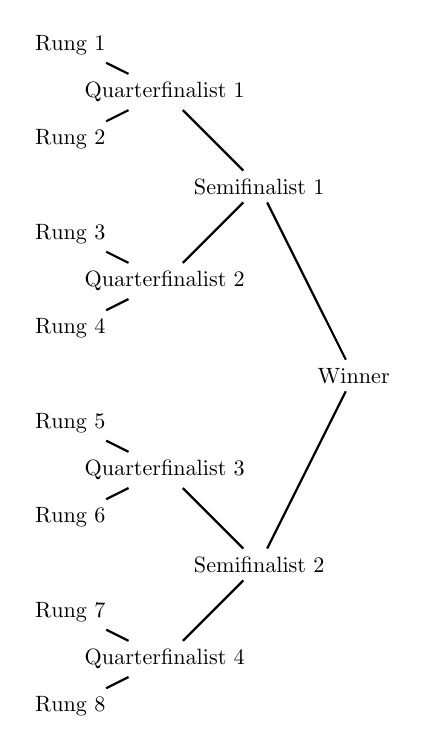
\begin{tikzpicture}[thick,scale=0.8, every node/.style={transform shape},grow'=left]
\node {Winner} 
  [sibling distance=6cm]
  child {node {Semifinalist 2}
  [sibling distance=3cm]
    child {node {Quarterfinalist 4}
    	    [sibling distance=1.5cm]
    	child {node {Rung 8}}
    	child {node {Rung 7}}
    }
    child {node {Quarterfinalist 3}
        [sibling distance=1.5cm]
    	child {node {Rung 6}}
    	child {node {Rung 5}}
    }
  }
  child {node {Semifinalist 1}
  [sibling distance=3cm]
    child {node {Quarterfinalist 2}
    [sibling distance=1.5cm]
    	child {node {Rung 4}}
    	child {node {Rung 3}}
    }
    child {node {Quarterfinalist 1}
        [sibling distance=1.5cm]
    	child {node {Rung 2}}
    	child {node {Rung 1}}
    }
  };
\end{tikzpicture}
\raisebox{4.4em}{\includegraphics[scale=0.8]{./images/tennisplayers}} 
\end{figure}


\end{frame}

%%%%%%%%%%%%%%%%%%%%%%%%%%%%%%%%%%%%%%%%
\begin{frame}
  \frametitle{Solution: Order Matters!}
  \begin{block}{Denominator}
	$8!$ basic outcomes -- ways to arrange players on tournament ladder.
  \end{block}
  \begin{block}{Numerator}
   Sequence of three decisions:
   \begin{enumerate}
    \item Which rung to put Federer on? (8 possibilities)
    \item Which rung to put Djokovic on? 
      \begin{itemize}
        \item For any given rung that Federer is on, only 4 rungs prevent Djokovic from meeting him until the final.
      \end{itemize}
    \item How to arrange the professors? ($6!$ ways)
   \end{enumerate}
  \end{block}
\alert{$$\frac{8 \times 4 \times 6!}{8!} = \frac{8\times 4}{7\times 8} = 4/7 \approx 0.57$$}

\end{frame}
%%%%%%%%%%%%%%%%%%%%%%%%%%%%%%%%%%%%%%%%
\begin{frame}

\centering \Huge Even if the basic outcomes are equally likely, the events of interest may not be...


\end{frame}
%%%%%%%%%%%%%%%%%%%%%%%%%%%%%%%%%%%%%%%%
\begin{frame}
\frametitle{``Odd Question'' \# 4}
To throw a total of 7 with a pair of dice, you have to get a 1 and a 6, or a 2 and a 5, or a 3 and a 4.
To throw a total of 6 with a pair of dice, you have to get a 1 and a 5, or a 2 and a 4, or a 3 and another 3.
	\vspace{1em}
	With two fair dice, you would expect:
		\begin{enumerate}[(a)]
			\item To throw 7 more frequently than 6.
			\item To throw six more frequently than 7.
			\item To throw 6 and 7 equally often.
		\end{enumerate}
\end{frame}
%%%%%%%%%%%%%%%%%%%%%%%%%%%%%%%%%%%%%%%%
\begin{frame}
\frametitle{Basic Outcomes Equally Likely, Events of Interest Aren't}

\begin{table}
	\begin{tabular}{|lr|cccccc|}
	\hline
	&&\multicolumn{6}{|c|}{Second Die}\\
	&&1&2&3&4&5&6\\
	\hline
	&1&2&3&4&5&\alert{6}&\textcolor{blue}{7}\\
	&2&3&4&5&\alert{6}&\textcolor{blue}{7}&8\\
	First&3&4&5&\alert{6}&\textcolor{blue}{7}&8&9\\
	Die&4&5&\alert{6}&\textcolor{blue}{7}&8&9&10\\
	&5&\alert{6}&\textcolor{blue}{7}&8&9&10&11\\
	&6&\textcolor{blue}{7}&8&9&10&11&12\\
	\hline
	\end{tabular}
	\caption{There are 36 equally likely basic outcomes, of which 5 correspond to a sum of six and 6 correspond to a sum of  seven.}
\end{table}
	\alert{$P(7) = 6/36 = 1/6$}\\
	\alert{$P(6) = 5/36$}
\end{frame}

\begin{singlespace}

\section{More Odd Questions}
%%%%%%%%%%%%%%%%%%%%%%%%%%%%%%%%%%%%%%%%
\begin{frame}
\frametitle{``Odd Question'' \# 6}
	\small
	You have been called to jury duty in a town where there are two taxi companies, Green Cab Ltd.\ 
	and Blue Taxi Inc. Blue taxi uses cars painted blue; Green Cabs uses green cars. Green cabs 
	dominates the market, with 85\% of the taxis on the road. On a misty winter night a taxi 
	sideswiped another car and drove off. A witness says it was a blue cab. The witness is tested 
	under conditions like those on the night of the accident, and 80\% of the time she correctly 
	reports the color of the cab that is seen. That is, regardless of whether she is shown a blue or a 
	green cab in misty evening light, she gets the color right 80\% of the time.

	You conclude, on the basis of this information:
	\begin{enumerate}[(a)]
		\item The probability that the sideswiper was blue is 0.8.
		\item It is more likely that the sideswiper was blue, but the probability is less than 0.8. 
		\item It is just as probable that the sideswiper was green as that it was blue. 
		\item It is more likely than not that the sideswiper was green.
	\end{enumerate}
\end{frame}

%%%%%%%%%%%%%%%%%%%%%%%%%%%%%%%%%%%%%%%%
\begin{frame}
\frametitle{``Odd Question'' \# 7}
	\small
	You are a physician. You think it is quite likely that one of your patients has strep throat, but you 
	aren't sure. You take some swabs from the throat and send them to a lab for testing. The test is 
	(like nearly all lab tests) not perfect. 
	\begin{itemize}
		\item If the patient has strep throat, then 70\% if the time the lab says yes. But 30\% of the 
		time it says NO.
		\item If the patient does not have strep throat, then 90\% of the time the lab says NO. But 
		10\% of the time it says YES.
	\end{itemize}
	You send five successive swabs to the lab, from the same patient. and get back these results in 
	order: YES, NO, YES, NO, YES. You conclude:
	\begin{enumerate}[(a)]
		\item These results are worthless.
		\item It is likely that the patient does not have strep throat.
		\item It is slightly more likely that the patient has strep throat.
		\item It is  much more likely that the patient has strep throat.
	\end{enumerate}
\end{frame}

\end{singlespace}

%%%%%%%%%%%%%%%%%%%%%%%%%%%%%%%%%%%%%%%%
\begin{frame}
\frametitle{Recall: Axioms of Probability}

Let $S$ be the sample space. With each event $A \subseteq S$ we associate a real number $P(A)$ called the \alert{probability of $A$}, satisfying the following conditions:
\vspace{1em}
\begin{description}
	\item[Axiom 1] $0 \leq P(A) \leq 1$ 
	\item[Axiom 2] $P(S)=1$
	\item[Axiom 3] If $A_1, A_2, A_3, \hdots$ are mutually exclusive events, then $P(A_1\cup A_2 \cup A_3 \cup \cdots) = P(A_1) + P(A_2) + P(A_3) + \hdots$
\end{description}

\end{frame}
%%%%%%%%%%%%%%%%%%%%%%%%%%%%%%%%%%%%%%%%
%\begin{frame}
%\frametitle{Key Point}
%The axoims of probability are out \emph{\alert{starting assumptions}} -- they are a complete description what we \emph{\alert{mean}} when we say ``probability.'' We use the axioms to derive various results for \emph{\alert{computing}} probabilities.
%\end{frame}
%
%%%%%%%%%%%%%%%%%%%%%%%%%%%%%%%%%%%%%%%%
%Some macros for the Venn Diagrams
\def\EventA{(-0.35,0) circle (1.2)}
\def\EventB{(1.35,0) circle (1.2)}
\def\EventC{(-0.35,0) circle (0.6)}
\def\EventD{(0,0) circle (1.6)}
\def\SampleSpace{(-2,-2) rectangle (3,2)}
%%%%%%%%%%%%%%%%%%%%%%%%%%%%%%%%%%%%%%%%
\begin{frame}
	\frametitle{The Complement Rule: $P(A^c) = 1- P(A)$}
	\begin{columns}
	
\column{0.7\textwidth}
\uncover<1->{Since $A, A^c$ are mutually exclusive and collectively exhaustive:}
$$\uncover<2->{P(A \cup A^c) =} \uncover<2->{P(A) + P(A^c) =} \uncover<3->{P(S) =} \uncover<3->{1}$$
\uncover<4->{Rearranging:}
	\uncover<4->{$$P(A^c) = 1 - P(A)$$}
\column{0.3\textwidth}
\uncover<1->{
\begin{figure}
\centering
\begin{tikzpicture}[scale = 0.6]
	\draw (1.8,0.8) node [above]{$A^c$};
	\draw \EventA node [above] {$A$};
      \draw \SampleSpace node [text=black,above] {$S$};
\end{tikzpicture}
\caption{$A\cap A^c = \emptyset$, $A \cup A^c = S$}
\end{figure}}

\end{columns}
\end{frame}
%%%%%%%%%%%%%%%%%%%%%%%%%%%%%%%%%%%%%%%%
\begin{frame}
\frametitle{Another Important Rule -- Equivalent Events}

\begin{block}{If A and B are Logically Equivalent, then $P(A) = P(B)$.}\end{block}

\begin{alertblock}{In other words, if A and B contain exactly the same basic outcomes, then $P(A) = P(B)$.}\end{alertblock}

Although this seems obvious it's important to keep in mind, especially later in the course...
\end{frame}
%%%%%%%%%%%%%%%%%%%%%%%%%%%%%%%%%%%%%%%%
\begin{frame}
\frametitle{The Logical Consequence Rule}

\begin{block}{If B Logically Entails A, then $P(B)\leq P(A)$}\end{block}

\begin{alertblock}{In other words, $B\subseteq A \Rightarrow P(B)\leq P(A)$}\end{alertblock}


\begin{block}{Why is this so?}
If $B \subseteq A$, then all the basic outcomes in $B$ are also in $A$.
\end{block}

\end{frame}
%%%%%%%%%%%%%%%%%%%%%%%%%%%%%%%%%%%%%%%%

\begin{frame}
\frametitle{Proof of Logical Consequence Rule (Optional)}
\framesubtitle{Proof won't be on a quiz or exam but is good practice with probability axioms.}
	\begin{columns}
	
\column{0.75\textwidth}
\uncover<1->{Since $B \subseteq A$, we have $B = A\cap B$ and $A = B \cup (A \cap B^c)$.}\uncover<1->{ Combining these,
	$$A = (A \cap B) \cup (A \cap B^c)$$}
\uncover<1->{Now since $(A \cap B) \cap (A \cap B^c) = \emptyset$,}
\begin{eqnarray*}
	\uncover<1->{P(A) &=& P(A \cap B)  + P(A \cap B^c)\\}
	\uncover<1->{&=&  P(B) + P(A \cap B^c)\\}
	\uncover<1->{&\geq& P(B)}
\end{eqnarray*}
\uncover<1->{because $0 \leq P(A \cap B^c) \leq 1$.}
\column{0.25\textwidth}
\uncover<1->{\begin{figure}
\centering
\begin{tikzpicture}[scale = 0.55]
	\draw \EventC;
	\draw \EventD;
	\draw (0, 0.5) node [above] {$A$};
	\draw (-0.3, -0.5) node [above] {$B$};
      \draw \SampleSpace node [text=black,above] {$S$};
\end{tikzpicture}
\caption{$B = A\cap B$, and $A = B \cup (A \cap B^c)$}
\end{figure}}

\end{columns}


\end{frame}
%%%%%%%%%%%%%%%%%%%%%%%%%%%%%%%%%%%%%%%%
\begin{frame}
\frametitle{``Odd Question'' \# 2}
\footnotesize
Pia is thirty-one years old, single, outspoken, and smart. She was a philosophy major. When a student, she was an ardent supporter of Native American rights, and she picketed a department store that had no facilities for nursing mothers. Rank the following statements in order from most probable to least probable.

	\vspace{1em}

		\begin{enumerate}[(A)]
			\item Pia is an active feminist.
			\item Pia is a bank teller.
			\item Pia works in a small bookstore.
			\item Pia is a bank teller and an active feminist.
			\item Pia is a bank teller and an active feminist who takes yoga classes.
			\item Pia works in a small bookstore and is an active feminist who takes yoga classes.
		\end{enumerate}
\end{frame}
%%%%%%%%%%%%%%%%%%%%%%%%%%%%%%%%%%%%%%%%
%\begin{frame}
%\frametitle{``Odd Question'' \# 2 -- Seven \emph{Events}}
%Write events D, E, and F in terms of A, B, C, and Y.
%		\begin{enumerate}[A]
%			\item = Pia is an active feminist.
%			\item = Pia is a bank teller.
%			\item = Pia works in a small bookstore.
%			\item[Y] = Pia takes yoga classes.\vspace{2em}
%			\item = Pia is a bank teller and an active feminist \pause \alert{$= A\cap B$}\pause
%			\item = Pia is a bank teller and an active feminist who takes yoga classes \pause \alert{$= A \cap B \cap Y$} \pause
%			\item = Pia works in a small bookstore and is an active feminist who takes yoga classes \pause \alert{$= A \cap C \cap Y$}
%		\end{enumerate}
%\end{frame}
%%%%%%%%%%%%%%%%%%%%%%%%%%%%%%%%%%%%%%%%
%\begin{frame}
%\frametitle{``Odd Question'' \# 2 -- Which Events are Subsets?}
%		\begin{enumerate}[A]
%			\item = Pia is an active feminist.
%			\item = Pia is a bank teller.
%			\item = Pia works in a small bookstore.
%			\item[Y] = Pia takes yoga classes.\vspace{2em}
%			\item $=A\cap B \pause \Rightarrow \alert{D\subseteq A,} \pause \alert{D\subseteq B}$\pause
%			\item $=A\cap B \cap Y\pause\Rightarrow \alert{E\subseteq D}$\pause
%			\item $=A\cap C \cap Y \pause \Rightarrow \alert{F \subseteq A,} \pause\alert{F \subseteq C}$
%		\end{enumerate}
%\end{frame}
%%%%%%%%%%%%%%%%%%%%%%%%%%%%%%%%%%%%%%%%%
%\begin{frame}
%\frametitle{``Odd Question'' \# 2 -- Apply Logical Consequence Rule}
%		\begin{enumerate}[A]
%			\item = Pia is an active feminist.
%			\item = Pia is a bank teller.
%			\item = Pia works in a small bookstore.
%			\item[Y] = Pia takes yoga classes.\vspace{2em}
%			\item $=A\cap B  \Rightarrow D\subseteq A, D\subseteq B \pause \Rightarrow \alert{P(D) \leq P(A), \pause P(D) \leq P(B)}$\pause
%			\item $=A\cap B \cap Y\Rightarrow E\subseteq D \pause \Rightarrow \alert{P(E) \leq P(D)}$\pause
%			\item $=A\cap C \cap Y \Rightarrow F \subseteq A, F \subseteq C \pause \Rightarrow \alert{P(F) \leq P(A), \pause P(F) \leq P(C)}$
%		\end{enumerate}
%\end{frame}
%%%%%%%%%%%%%%%%%%%%%%%%%%%%%%%%%%%%%%%%
\begin{frame}
\frametitle{Using the Logical Consequence Rule...}
 \footnotesize
		\begin{enumerate}[(A)]
			\item Pia is an active feminist.
			\item Pia is a bank teller.
			\item Pia works in a small bookstore.
			\item Pia is a bank teller and an active feminist.
			\item Pia is a bank teller and an active feminist who takes yoga classes.
			\item Pia works in a small bookstore and is an active feminist who takes yoga classes.
		\end{enumerate}
\begin{alertblock}{Any Correct Ranking Must Satisfy:}\end{alertblock}
\begin{eqnarray*}
P\mbox{(A)}\geq P\mbox{(D)}\geq P\mbox{(E)}\\
P\mbox{(B)}\geq P\mbox{(D)}\geq P\mbox{(E)}\\
P\mbox{(A)}\geq P\mbox{(F)}\\
P\mbox{(C)}\geq P\mbox{(F)}
\end{eqnarray*}
\end{frame}
%%%%%%%%%%%%%%%%%%%%%%%%%%%%%%%%%%%%%%%%
\begin{frame}
\frametitle{Throw a Fair Die Once}
\begin{block}{$E = $ roll an even number}
\end{block}
\begin{block}{What are the basic outcomes?}
$\{1,2,3,4,5,6\}$
\end{block}\pause
\begin{block}{What is $P(E)$? }\pause
$E = \{2,4,6\}$ and the basic outcomes are equally likely (and mutually exclusive), so 
	$$P(E) = 1/6 + 1/6 + 1/6 = 3/6 = \alert{1/2}$$
\end{block}

\end{frame}
%%%%%%%%%%%%%%%%%%%%%%%%%%%%%%%%%%%%%%%%
\begin{frame}
\frametitle{Throw a Fair Die Once}
\begin{block}{$E = $ roll an even number \hfill $M = $ roll a 1 or a prime number}
\end{block}
\begin{alertblock}{What is $P(E\cup M)$?}\end{alertblock}
\pause
Key point: $E$ and $M$ are not mutually exclusive! 
	\begin{eqnarray*}
		P(E\cup M) &=& P(\{1,2,3,4,5,6\})= 1\\ 
		P(E) &=& P(\{2,4,6\}) = 1/2\\ 
		P(M) &=& P(\{1,2,3,5\}) = 4/6 = 2/3\\ \\
		P(E) + P(M) &=& 1/2 + 2/3 = 7/6 \neq P(E\cup M) = 1
	\end{eqnarray*}

\end{frame}
%%%%%%%%%%%%%%%%%%%%%%%%%%%%%%%%%%%%%%%%


\begin{frame}
\frametitle{The Addition Rule -- Don't Double-Count!}
$$P(A\cup B) = P(A) + P(B) - P(A\cap B)$$
\begin{figure}
\centering
\begin{tikzpicture}[scale = 1.2]

	\begin{scope}[fill opacity = 0.5]
		\fill[blue] \EventA;
		\fill[red] \EventB;
	\end{scope}
	
	\draw \EventA node [above] {$A$};
	\draw \EventB node [above] {$B$};
      \draw \SampleSpace node [text=black,right] {$S$};
\end{tikzpicture}
\end{figure}
\alert{Construct a formal proof as an optional homework problem.}
\end{frame}
%%%%%%%%%%%%%%%%%%%%%%%%%%%%%%%%%%%%%%%%
\begin{frame}
\begin{center}\Huge Who's on the other side?\end{center}
\end{frame}
%%%%%%%%%%%%%%%%%%%%%%%%%%%%%%%%%%%%%%%%
\begin{frame}
\frametitle{Three Cards, Each with a Face on the Front and Back}
\begin{figure}
\fbox{\includegraphics[scale = 0.75]{./images/gaga}}
\hspace{1em}
\fbox{\includegraphics[scale = 0.75]{./images/obama}}
\end{figure}
\begin{enumerate}
	\item Gaga/Gaga
	\item Obama/Gaga
	\item Obama/Obama
\end{enumerate} 
\begin{alertblock}{I draw a card at random and look at one side: it's Obama. What is the probability that the other side is also Obama?\\\hfill}\end{alertblock}
\end{frame}
%%%%%%%%%%%%%%%%%%%%%%%%%%%%%%%%%%%%%%%%
\begin{frame}
\frametitle{Let's Try The Method of Monte Carlo...}
\framesubtitle{When you don't know how to calculate, simulate.}
Procedure
\begin{enumerate}
\item Close your eyes and thoroughly shuffle your cards.
\item Keeping eyes closed, draw a card and place it on your desk.
\item Stand if Obama is face-up on your chosen card. 
\item We'll count those standing and call the total $N$
\item Of those standing, sit down if Obama is \emph{not} on the back of your chosen card.
\item We'll count those \emph{still} standing and call the total $m$.
\end{enumerate}

\begin{alertblock}{Monte Carlo Approximation of Desired Probability $\displaystyle= \frac{m}{N}$}\end{alertblock}
\end{frame}
%%%%%%%%%%%%%%%%%%%%%%%%%%%%%%%%%%%%%%%%
\begin{frame}

% Set the overall layout of the tree
\tikzstyle{level 1}=[level distance=3.5cm, sibling distance=3.5cm]
\tikzstyle{level 2}=[level distance=3.5cm, sibling distance=2cm]

% Define styles for bags and leafs
\tikzstyle{bag} = [text width=4em, text centered]
\tikzstyle{end} = [circle, minimum width=3pt,fill, inner sep=0pt]


\begin{tikzpicture}[thick,scale=0.94, every node/.style={transform shape},grow=right]
\node[bag]{Choose Card}
    child {
        node[bag] {Obama Obama}        
        child {
                node[end, label=right:
                    {Obama}] {}
                edge from parent
                node[below]  {$\frac{1}{2}$}
            }
            child {
                node[end, label=right:
                    {Obama}] {}
                edge from parent
                node[above] {$\frac{1}{2}$}
            }
            edge from parent 
            node[below]  {$\frac{1}{3}$}
    }
        child {
        node[bag] {Obama Gaga}        
        child {
                node[end, label=right:
                    {Gaga}] {}
                edge from parent
                node[below]  {$\frac{1}{2}$}
            }
            child {
                node[end, label=right:
                    {Obama}] {}
                edge from parent
                node[above] {$\frac{1}{2}$}
            }
            edge from parent 
            node[above]{$\frac{1}{3}$}
    }
    child {
        node[bag] {Gaga Gaga}        
        child {
                node[end, label=right:
                    {Gaga}] {}
                edge from parent
                node[below]  {$\frac{1}{2}$}
            }
            child {
                node[end, label=right:
                    {Gaga}] {}
                edge from parent
                node[above] {$\frac{1}{2}$}
            }
        edge from parent         
            node[above] {$\frac{1}{3}$}
    };
\end{tikzpicture}

\end{frame}
%%%%%%%%%%%%%%%%%%%%%%%%%%%%%%%%%%%%%%%%
\begin{frame}
\frametitle{Conditional Probability -- Reduced Sample Space}
\framesubtitle{Set of relevant outcomes restricted by condition}
$$P(A|B) = \frac{P(A\cap B)}{P(B)},\;\; \mbox{provided } P(B)>0$$
\begin{figure}
\centering
\begin{tikzpicture}[scale = 1]

	\begin{scope}[fill opacity = 0.5]
		\fill[red] \EventB;
      	\clip \EventA;
      	\fill[blue] \EventB;
    \end{scope}
	\draw \EventA node [above] {$A$};
	\draw \EventB node [above] {$B$};
      \draw \SampleSpace node [right] {$S$};
\end{tikzpicture}
\caption{$B$ becomes the ``new sample space'' so we need to re-scale by $P(B)$ to keep probabilities between zero and one.}
\end{figure}
\end{frame}
%%%%%%%%%%%%%%%%%%%%%%%%%%%%%%%%%%%%%%%%
\begin{frame}
\frametitle{Who's on the other side?}
Let $F$ be the event that Obama is on the front of the card of the card we draw and $B$ be the event that he is on the back.
$$P(B|F) = \frac{P(B\cap F)}{P(F)} = \pause \alert{\frac{1/3}{1/2}= \pause 2/3}$$

\end{frame}

%%%%%%%%%%%%%%%%%%%%%%%%%%%%%%%%%%%%%%%%
\begin{frame}
  \small
  \begin{block}{Conditional Versions of Probability Axioms}
    \begin{enumerate}
      \item $0 \leq P(A|B) \leq 1$
      \item $P(B|B) = 1$
      \item If $A_1, A_2, A_3, \dots$ are mutually exclusive events, then $P(A_1\cup A_2\cup A_3 \cup \cdots|B) = P(A_1|B) + P(A_2|B) + P(A_3|B)\dots$
    \end{enumerate}
  \end{block}

  \begin{block}{Conditional Versions of Other Probability Rules}
    \begin{itemize}
      \item $P(A|B) = 1 - P(A^c|B)$
      \item $A_1$ logically equivalent to $A_2 \iff P(A_1|B) = P(A_2|B)$
      \item $A_1 \subseteq A_2 \implies P(A_1|B) \leq P(A_2|B)$  
      \item $P(A_1 \cup A_2 | B) = P(A_1|B) + P(A_2|B) - P(A_1 \cap A_2|B)$
    \end{itemize}
  \end{block}


    \alert{However: $P(A|B) \neq P(B|A)$ and $P(A|B^c) \neq 1 - P(A|B)$!}
  
\end{frame}
%%%%%%%%%%%%%%%%%%%%%%%%%%%%%%%%%%%%%%%%
\begin{frame}
\frametitle{Independence and The Multiplication Rule}
\begin{block}{The Multiplication Rule}
Rearrange the definition of conditional probability:
$P(A\cap B) = P(A|B)P(B)$
\end{block}\pause
\begin{block}{Statistical Independence}
$P(A\cap B) = P(A)P(B)$
\end{block}\pause
\begin{alertblock}{By the Multiplication Rule}
$\mbox{Independence } \iff P(A|B) = P(A)$\\
\end{alertblock}\pause
\begin{block}{Interpreting Independence}
Knowledge that $B$ has occurred tells nothing about whether $A$ will.
\end{block}
\end{frame}
%%%%%%%%%%%%%%%%%%%%%%%%%%%%%%%%%%%%%%%%

\begin{frame}
\frametitle{Will Having 5 Children Guarantee a Boy? }
A couple plans to have five children. Assuming that each birth is independent and male and female children are equally likely, what is the probability that they have at least one boy?
\vspace{1em}

\pause
\alert{By Independence and the Complement Rule,}
	\begin{eqnarray*}
		P(\mbox{no boys})&=& P(\mbox{5 girls})\\
							&=& 1/2 \times 1/2 \times 1/2 \times 1/2 \times 1/2\\
							&=&\ 1/32\\ \\ \pause
		P(\mbox{at least 1 boy})&=&1 - P(\mbox{no boys})\\
		&=&1 - 1/32 =31/32 = 0.97
	\end{eqnarray*}

\end{frame}
%%%%%%%%%%%%%%%%%%%%%%%%%%%%%%%%%%%%%%%%
%
%\begin{frame}
%\frametitle{An Example -- Do you agree with this calculation? }
%\begin{quote}
%	On September 9, 1982, the four-digit lottery number 8092 was drawn in both Massachusetts and New Hampshire. This was described as a 1 in 100 million event.
%\end{quote}
%\vspace{1em}
%\alert{10,000 possible draws, equally likely, independent $\Rightarrow \mbox{Prob}=1/(10,000)(10,000)=$ 1 in 100 Million}
%\vspace{1em}
%\begin{enumerate}[(a)]
%	\item Agree
%	\item Disagree
%\end{enumerate}
%
%\end{frame}
%%%%%%%%%%%%%%%%%%%%%%%%%%%%%%%%%%%%%%%%%
%\begin{frame}
%\frametitle{What Probability Should we Calculate?}
%\pause
%\begin{block}{A = Both draw 8092 on \emph{particular day}}
%	$P(A) = 1/(10000) \times 1/(10000)  = $ 1 in 100 Million
%\end{block}
%\pause
%\begin{block}{B = Both draw \emph{same number} on \emph{particular day}}
%	10,000 mutually exclusive numbers to match on $P(B) = 10000 \times P(A) =$ 1 in 10 Thousand
%\end{block}
%\pause
%\begin{block}{C = Same draw in NH/MA at least once over 3 years}
%3 Years $\approx$ 1000 Days 
%\end{block}
%\pause
%\begin{block}{D = Same draw in \emph{some} pair of states at least once in 3 years}
%${52 \choose 2} = 1225$ pairs of states 
%\end{block}
%\pause
%\hfill \alert{\fbox{How to calculate $P(C)$?}}
%
%\end{frame}
%%%%%%%%%%%%%%%%%%%%%%%%%%%%%%%%%%%%%%%%%
%\begin{frame}
%	\frametitle{C = Same draw in NH/MA at least once over 3 years}
%\begin{block}{Complement Rule (and Independence)}
%	\begin{eqnarray*}
%	P(C) &=&\pause 1 - P(\mbox{No day with same draw over 1000 days})\\
%		&=&\pause 1 - P(\mbox{both draw different number on particular day})^{1000}\\
%		&=&\pause 1 - \left[1 - P(B)  \right]^{1000}\\
%		&=&\pause 1 - (9999/10000)^{1000}\\
%		&=&\pause 1 - (0.9999)^{1000}\\
%		&\approx&\pause 1 - 0.9 \pause = 0.1
%	\end{eqnarray*}
%	\alert{In other words, $P(C) \approx$ 1 in 10}
%\end{block}
%
%\end{frame}
%%%%%%%%%%%%%%%%%%%%%%%%%%%%%%%%%%%%%%%%%
%\begin{frame}
%	\frametitle{D = Same draw \emph{some} pair of states at least once in 3 years}
%		The calculation is more involved for this example so we won't go through it here. However, it is clear that $P(D)$ will be \emph{\alert{much larger}} than $P(C) \approx 1/10$ because there are 1225 pairs of states.
%		
%\end{frame}
%%%%%%%%%%%%%%%%%%%%%%%%%%%%%%%%%%%%%%%%%
%\begin{frame}
%\frametitle{Bottom Line:}
%
%
% It \emph{is} surprising that the number 8092 was drawn in MA and NH on September 9, 1982. It is \emph{not} surprising, however, that two states will sometimes draw the same lottery number. Since the newspaper would have reported a match between \emph{\alert{any}} states on \emph{\alert{any}} day involving \emph{\alert{any}} lottery number, the probability they give is not the relevant one.
%
%\end{frame}
%%%%%%%%%%%%%%%%%%%%%%%%%%%%%%%%%%%%%%%%%
%
%\begin{frame}
%\frametitle{The Birthday Problem (Optional Homework Question)}
%	\begin{quote}
%		What is the least number of persons required if the probability exceeds 1/2 that two or more of them have the same birthday? (Year of birth need not match.)
%	\end{quote}
%	
%	\hfill \alert{[Hint: Use the Complement Rule.]}
%\end{frame}
%
%%%%%%%%%%%%%%%%%%%%%%%%%%%%%%%%%%%%%%%%%



\begin{frame}
\frametitle{The Law of Total Probability}
If $E_1, E_2, \hdots, E_k$ are mutually exclusive, collectively exhaustive events and $A$ is another event, then
	$$P(A) = P(A|E_1)P(E_1) + P(A|E_2)P(E_2) + \hdots + P(A|E_k)P(E_k)$$

\end{frame}
%%%%%%%%%%%%%%%%%%%%%%%%%%%%%%%%%%%%%%%%
\begin{frame}
  \frametitle{Example of Law of Total Probability}
  Define the following events:
  \begin{eqnarray*}
    F &=&  \mbox{Obama on front of card}\\
    A &=&  \mbox{Draw card with two Gagas}\\
    B &=&  \mbox{Draw card with two Obamas}\\
    C &=&  \mbox{Draw card with BOTH Obama and Gaga}\\
  \end{eqnarray*}
  \begin{eqnarray*}
  P(F) &=& P(F|A)P(A) + P(F|B)P(B) + P(F|C)P(C) \\ \pause
  &=& 0 \times 1/3 + 1 \times 1/3 + 1/2 \times 1/3 \\
  &=& 1/2
  \end{eqnarray*}

\end{frame}
%%%%%%%%%%%%%%%%%%%%%%%%%%%%%%%%%%%%%%%%
%Some macros for the Venn Diagrams
\def\EventA{(-0.35,0) circle (1.2)}
\def\EventB{(1.35,0) circle (1.2)}
\def\EventC{(-0.35,0) circle (0.6)}
\def\EventD{(0,0) circle (1.6)}
\def\SampleSpace{(-2,-2) rectangle (3,2)}
%%%%%%%%%%%%%%%%%%%%%%%%%%%%%%%%%%%%%%%%
\begin{frame}
\frametitle{Deriving the Law of Total Probability For $k=2$}
\framesubtitle{You are responsible for this proof on quizzes and exams.}

\begin{columns}

\column{0.7\textwidth}
\uncover<2->{

Since $A\cap B$ and $A \cap B^c$ are mutually exclusive and their union equals $A$,
	$$P(A) = P(A\cap B) + P(A \cap B^c)$$}
	\uncover<3->{
But by the multiplication rule:
	\begin{eqnarray*}
		P(A\cap B)&=&P(A|B)P(B)\\
		P(A \cap B^c)&=&P(A|B^c)P(B^c)
	\end{eqnarray*}}
\uncover<4->{
Combining,
	$$\alert{P(A) = P(A|B)P(B) + P(A|B^c)P(B^c)}$$}
\column{0.3\textwidth}
\uncover<1->{
\begin{figure}
\centering
\begin{tikzpicture}[scale = 0.5]

	\begin{scope}[fill opacity = 0.5]
		\fill[red] \EventB;
      	\clip \EventA;
      	\fill[blue] \EventB;
    \end{scope}
	\draw \EventA node [above] {$B$};
	\draw \EventB node [above] {$A$};
      \draw \SampleSpace node [right] {$S$};
\end{tikzpicture}
\caption{$A = (A\cap B) \cup (A \cap B^c)$, $(A\cap B) \cap (A \cap B^c) = \emptyset$}
\end{figure}}

\end{columns}

\end{frame}
%%%%%%%%%%%%%%%%%%%%%%%%%%%%%%%%%%%%%%%%

\begin{frame}

\frametitle{How do prediction markets work?}
\framesubtitle{To learn more, see \fbox{\href{http://www.aeaweb.org/articles.php?doi=10.1257/0895330041371321}{Wolfers \& Zitzewitz (2004)}}}
\begin{center}
\fbox{\fbox{\begin{minipage}{0.6\textwidth}
  \textsc{This certificate entitles the bearer to \$1 if Trump wins the 2016 US presidential election.}
\end{minipage}}}
\vspace{1em}

\begin{block}{Buyers -- Purchase Right to Collect}
Trump very likely to win $\Rightarrow$ buy for close to \$1. \\Trump very unlikely to win $\Rightarrow$ buy for close to \$0.
\end{block}

\begin{block}{Sellers -- Sell Obligation to Pay} 
Trump very likely to win $\Rightarrow$ sell for close to \$1. \\Trump very unlikely to win $\Rightarrow$ sell for close to \$0.
\end{block}
\end{center}

\end{frame}
%%%%%%%%%%%%%%%%%%%%%%%%%%%%%%%%%%%%%%%%
\begin{frame}

  \begin{block}{Probabilities from Beliefs}
    Market price of contract encodes market participants' beliefs in the form of probability:
$$\mbox{Price}/\mbox{Payout}\approx \mbox{Subjective Probability}$$
  \end{block} \pause

	\begin{alertblock}{Statistical Arbitrage}
    If the probabilities implied by prediction market prices violate \emph{any} of our probability rules there is a \emph{pure arbitrage opportunity}: a way make to make a guaranteed, risk-free profit.
	\end{alertblock} \pause

  \vspace{1em}
  \alert{Last I checked a \$1 contract on Trump winning was going for \$0.29 on \url{predictit.org}}
\end{frame}
%%%%%%%%%%%%%%%%%%%%%%%%%%%%%%%%%%%%%%%%
\begin{frame}
\frametitle{A Simple Example of Statistical Arbitrage}
\framesubtitle{Courtesy of  \fbox{\href{http://offsettingbehaviour.blogspot.co.nz/2012/11/barriers-to-arbitrage.html}{Eric Crampton}}}

\begin{block}{November 5th, 2012}
	\begin{itemize}
		\item\$2.30 for contract paying \$10 if Romney wins on BetFair
		\item \$6.58 for contract paying \$10 if Obama wins on InTrade
	\end{itemize}
\end{block}

\begin{block}{Implied Probabilities}
	\begin{itemize}
	\item BetFair: $P(Romney) \approx 0.23$
	\item InTrade: $P(Obama) \approx 0.66$
	\end{itemize}
\end{block}

\begin{alertblock}{What's Wrong with This?}\pause
 Violates complement rule! $P(Obama) = 1 - P(Romney)$ but the implied probabilities here don't sum up to one!
\end{alertblock}



\end{frame}

%%%%%%%%%%%%%%%%%%%%%%%%%%%%%%%%%%%%%%%%
\begin{frame}
\frametitle{A Simple Example of Statistical Arbitrage}
\framesubtitle{Courtesy of  \fbox{\href{http://offsettingbehaviour.blogspot.co.nz/2012/11/barriers-to-arbitrage.html}{Eric Crampton}}}

\begin{block}{November 5th, 2012}
	\begin{itemize}
		\item\$2.30 for contract paying \$10 if Romney wins on BetFair
		\item \$6.58 for contract paying \$10 if Obama wins on InTrade
	\end{itemize}
\end{block}

\begin{alertblock}{Arbitrage Strategy}
Buy Equal Numbers of Each 
	\begin{itemize}
		\item Cost = \$2.30 + \$6.58 =\$8.88 per pair 
		\item Payout if Romney Wins: \$10 
		\item Payout if Obama Wins: \$10
		\item Guaranteed Profit: \$10 - \$8.88 = \$1.12 per pair
	\end{itemize} 

\end{alertblock}



\end{frame}
%%%%%%%%%%%%%%%%%%%%%%%%%%%%%%%%%%%%%%%%
\end{document}
